\section{Context} 

Inversions, as defined by HGVS \cite{noauthor_inversion_nodate} (Human Genome Variation Society), are sequence changes where, compared to a reference sequence, more than one nucleotide replacing the original sequence is the reverse complement of the original sequence. They are a category of genomic structural variations (SVs), defined as alterations in the DNA that affect more than 50 bp that may delete, insert, duplicate, invert, or move genomic sequences \cite{eslami_rasekh_discovery_2017} (see Figure \ref{fig:svs}). 

\begin{figure}[h]

  \centering
    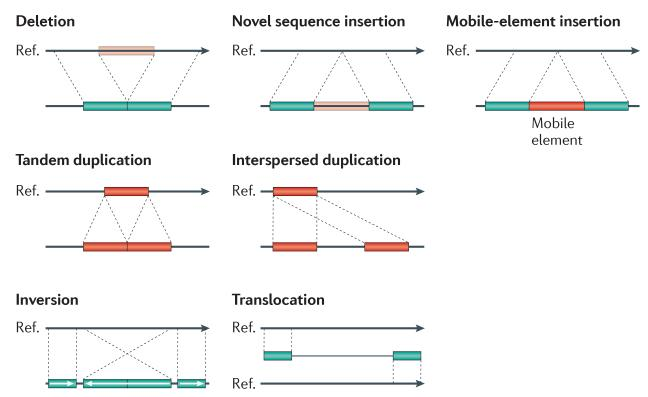
\includegraphics[width=250px]{svs.jpg}

  \caption{Outline of different SV-archetypes.}
  \label{fig:svs}
\end{figure}

They are often generated by non-allelic homologous recombination (NAHR) between inverted repeats, but they can also be originated by double-strand break repair mechanisms, like non-homologous end joining (NHEJ), or replication-based mechanisms mediated by microhomology, like fork stalling and template switching \cite{puig_human_2015}. Although inversions constitute only a small fraction of SVs across various organisms, ranging from 0.5\% to 7\% \cite{hu_unravelling_2024}, they can span over 100 Mb and collectively account for up to 10\% of the genome, holding considerable functional and evolutionary significance. \\


Inversions were first identified in 1917 by Alfred Sturtevant \cite{sturtevant_case_1921}, and he found out they act as suppressors of recombination between chromosomes. Since then, inversions have been drawing increasing attention, due to their crucial role in driving genome evolution and their link to the evolutionary processes of many species. In fact, it was later found that suppressed recombination among genes within an inversion can lead to largely independent genome evolution between derived and ancestral arrangements, providing opportunities for divergence and speciation \cite{faria_evolving_2019}. This genomic isolation, facilitated by inversions, can lead to the formation of novel genotypes and phenotypes, contributing to the genetic diversity we can observe today. \\

But inversions are not only related to evolution. In fact, they are involved in the formation of several diseases, as will be shown in Chapter 2. A recent study even shows that the contribution of chromosomal inversions to phenotypic diversity can even affect brain development and lead to disorders \cite{wang_chromosomal_2023}.

\section{Inversions detection}

Due to their significance, the challenge of detecting inversions has been widely addressed. The first methods developed for this scope, such as cytogenetics or PCR-based approaches, were labor‐intensive and lacked resolution, limiting their effectiveness \cite{hu_unravelling_2024}. With the advent of high-throughput next-generation sequencing (NGS), large-scale population studies of inversions became finally possible, enabling the discovery of polymorphic inversions and their association with phenotypic traits.
In addition to this, long‐read DNA sequencing technologies such as PacBio HiFi sequencing or Oxford Nanopore duplex sequencing have enabled the generation of sequencing reads between 10  kb and 2  Mb, making them highly useful for detecting inversions. Therefore, identifying inversions has become more straightforward with the use of long reads that can span repetitive and complex genomic regions. However, despite all this technological progress, inversions remain one of the most underascertained forms of structural variation in human and non-human primate genomes, limiting our understanding of their evolution significance \cite{porubsky_recurrent_2020}. The main challenge continues to be the precise determination of inversion breakpoints.

\section{Project}

In this thesis will be presented an algorithm designed to detect the presence of genomic inversions from long-read sequencing data using sample-specific strings (which will be defined in detail in Chapter 2) to determine the breakpoints. A \texttt{Python} implementation of the algorithm will be used for the practical experimentation, in combination with the SVDSS \cite{denti_svdss_2023} tool, that will also be implemented in the code and will help in detecting the number, position, and length of the sample-specific strings. \\
\\
In Chapter 2, the necessary preliminaries will be presented to understand how the algorithm works, including the definitions used throughout the thesis and the biological background that lies behind inversions, other than their pratical biological consequences. \\
In Chapter 3, the algorithm will be presented in detail, including the pseudocode and a complete theoretical analysis. This chapter will treat, among other things, time and space complexity and proof of correctness.\\
In Chapter 4, the practical experimentation will be discussed, explaining the \texttt{Python} implementation of the code and the use of the SVDSS tool. The results will be presented, summarized, and commented upon.

\bigskip
\bigskip

